\documentclass[11pt,a4paper,openany]{book}
\usepackage[margin=24mm]{geometry}
\usepackage{fontspec}
\IfFontExistsTF{Noto Serif}{\setmainfont{Noto Serif}}{\setmainfont{DejaVu Serif}}
\usepackage{amsmath,amssymb,tikz,enumitem,microtype}
\usepackage[hidelinks]{hyperref}
\setlength{\parindent}{0pt}
\setlength{\parskip}{6pt}
\setlist[enumerate]{leftmargin=*,itemsep=8pt}
\setlength{\emergencystretch}{2em}

\renewcommand{\contentsname}{Mục lục}
\begin{document}
\title{V-TALENT 2045\\ PHY201-A --- Vector, giải tích và xấp xỉ dành cho Vật lý\\\large Level 2 \textbar{} Mathematics for Physics}
\author{Dr. Dang Minh Tuan -- TS. Đặng Minh Tuấn}
\date{2026 \textbar{} Draft v1.0}
\maketitle
\tableofcontents
\chapter*{Hướng dẫn học}
Lớp 10–12 / chuyển tiếp Olympic. Tiên quyết: đại số, lượng giác, hình học tọa độ và PHY101-A. Giải tích phát triển từ ý nghĩa vật lý; ODE và số phức tiếp tục ở PHY201-B.

Đọc mục tiêu và trả lời câu chẩn đoán trước lý thuyết. Tự tái lập lời giải ví dụ, giải độc lập bài luyện tập rồi dùng lời giải cuối sách để chẩn đoán lỗi. Dùng sổ riêng ghi dự đoán, sơ đồ và kiểm tra. Nội dung và bài tập tự biên soạn; nguồn ngoài là chỉ dẫn đọc, không sao chép. Bản thảo chờ thẩm định độc lập.
\chapter{Vector, phép chiếu và các tích vật lý}
\section{Mục tiêu và chẩn đoán}
Phân tích vector, dùng tích vô hướng và có hướng kèm đơn vị, xác định ràng buộc hình học.

\textbf{Dự đoán:} Lực khác 0 có thể không sinh công? Lực khác 0 có thể không tạo moment không?
\section{Lý thuyết và suy dẫn}
Vector không chỉ là danh sách số: thành phần phụ thuộc cơ sở. Trong hệ Descartes trực chuẩn, $\vec a=a_x\hat e_x+a_y\hat e_y+a_z\hat e_z$, $|\vec a|=\sqrt{a_x^2+a_y^2+a_z^2}$. Vector đơn vị $\hat n$ có độ lớn một. Hình chiếu vô hướng $\vec a\cdot\hat n$ có dấu, hình chiếu vector $(\vec a\cdot\hat n)\hat n$. Phần vuông góc $\vec a-(\vec a\cdot\hat n)\hat n$. Phân tích này là nền tảng của sơ đồ lực, động học thành phần và đo trường.

Tích vô hướng thỏa $\vec a\cdot\vec b=a_xb_x+a_yb_y+a_zb_z=ab\cos\theta$. Suy dạng hình học bằng khai triển $|\vec a-\vec b|^2$ rồi đối chiếu định lý cos. Công lực không đổi $W=\vec F\cdot\Delta\vec r$; công suất tức thời $P=\vec F\cdot\vec v$. Cả hai là vô hướng có dấu. Lực vuông góc độ dời không sinh công, nhưng có thể đổi hướng vận tốc.

Trong cơ sở thuận, $\vec a\times\vec b=(a_yb_z-a_zb_y,\ a_zb_x-a_xb_z,\ a_xb_y-a_yb_x)$. Độ lớn $ab\sin\theta$, hướng theo quy tắc bàn tay phải. Tích phản đối xứng: $\vec b\times\vec a=-\vec a\times\vec b$. Moment lực đối với gốc xác định là $\vec\tau=\vec r\times\vec F$; lực từ $\vec F=q\vec v\times\vec B$. Moment phụ thuộc gốc chọn. Lực từ vuông góc vận tốc, riêng nó không đổi động năng trong cơ học cổ điển.

Với phương trình vector, chiếu lên các hướng độc lập để thu phương trình vô hướng. Chọn trục theo mặt phẳng hoặc liên kết thường đơn giản hóa mô hình. Trong ba chiều, thành phần moment quanh trục đơn vị $\hat n$ là $\tau_n=(\vec r\times\vec F)\cdot\hat n$. Không nhầm độ lớn moment tổng với thành phần quanh một bản lề cụ thể.
\begin{center}
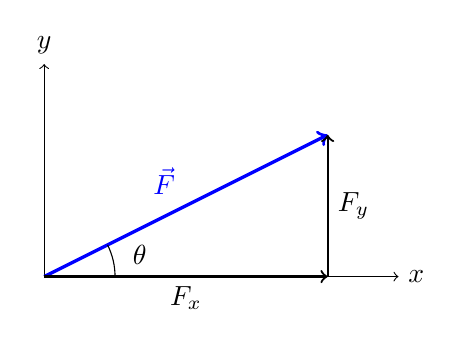
\begin{tikzpicture}[scale=.9]\draw[->](0,0)--(5,0)node[right]{$x$};\draw[->](0,0)--(0,3)node[above]{$y$};\draw[->,very thick,blue](0,0)--node[above left]{$\vec F$}(4,2);\draw[dashed](4,2)--(4,0);\draw[->,thick](0,0)--node[below]{$F_x$}(4,0);\draw[->,thick](4,0)--node[right]{$F_y$}(4,2);\draw (1,0) arc(0:26.565:1);\node at (1.35,.3){$\theta$};\end{tikzpicture}
\end{center}
\section{Ví dụ có lời giải}
\subsection*{Ví dụ 1.1}
Lực F=(3,-4,2) N làm vật dịch chuyển d=(2,1,-1) m. Tìm công và góc giữa hai vector.

\textbf{Lời giải.} $W=6-4-2=0$ J. Hai vector khác 0 nên $\cos\theta=0$, $\theta=90^\circ$. Lực khác 0 có thể không sinh công trên độ dời.
\subsection*{Ví dụ 1.2}
Lực (0,5,0) N đặt tại r=(0,3;0;0,4) m. Tính moment và thành phần z.

\textbf{Lời giải.} $\vec\tau=(-2,0,1{,}5)$ N m; $\tau_z=1{,}5$ N m. Độ lớn $\sqrt{4+2{,}25}=2{,}5$ N m. Bản lề trục z liên quan thành phần z, không phải độ lớn tổng.
\subsection*{Ví dụ 1.3}
Phân tích trọng lực theo phương dọc và vuông góc dốc nhẵn 30\textdegree{} với vật 2 kg (g=9,81).

\textbf{Lời giải.} Thành phần xuống dốc $mg\sin30^\circ=9{,}81$ N; ép vào mặt $mg\cos30^\circ\approx16{,}99$ N. Phản lực 16,99 N nếu không có gia tốc hay lực khác theo pháp tuyến.
\section{Nhiệm vụ thực nghiệm}
Dùng thước nhẹ có trục gần một đầu và quả cân nhỏ. Dự đoán moment theo cánh tay đòn vuông góc; so sánh các cấu hình cân bằng. Giữ trục cố định, không dùng tải nặng.
\section{Ứng dụng hiện đại và chuyển giao}
Khớp robot tại gốc chịu tải tại $\vec r=(0{,}4,0{,}2,0)$ m với lực $\vec F=(0,-30,0)$ N. Moment $(0,0,-12)$ N m. Động cơ phải cân bằng moment tĩnh này cùng các tải khác. Chuyển giao: so sánh đổi cánh tay đòn vuông góc và đổi hướng lực; giải thích vì sao cùng lực có thể đòi hỏi moment truyền động rất khác.
\section{Chỉ dẫn đọc nguồn}
SW-1.1.1 and SW-1.1.2: pp. 13–18; SJ-05: ch. 5, pp. 20–24; SJ-17: torque and angular momentum, pp. 68–73.
\section{Luyện tập độc lập}
\begin{enumerate}
\item \textbf{PHY201-A-1.1}. Tìm hình chiếu của a=(4,3,0) lên vector đơn vị n=(3/5,4/5,0).
\item \textbf{PHY201-A-1.2}. Tìm a\ensuremath{\times}b với a=(1,2,3), b=(0,1,-1), rồi kiểm tra vuông góc.
\item \textbf{PHY201-A-1.3}. Lực (5,-2,0) N tác dụng khi vận tốc (-1,4,0) m/s. Tìm công suất tức thời và ý nghĩa dấu.
\item \textbf{PHY201-A-1.4}. Điện tích dương 2 \ensuremath{\mu}C chuyển động với (3000,0,0) m/s trong B=(0,0,0,2) T. Tìm lực từ.
\item \textbf{PHY201-A-1.5}. Với r=(0,2;0,3;0) m và F=(10,0,0) N, tìm moment quanh gốc và quanh điểm O\ensuremath{\prime}=(0;0,3;0).
\end{enumerate}
\chapter{Đạo hàm: tốc độ biến thiên, cực trị và mô hình cục bộ}
\section{Mục tiêu và chẩn đoán}
Suy ra vận tốc và gia tốc, dùng quy tắc hàm hợp/tích và kiểm tra cực trị cùng biên miền xác định.

\textbf{Dự đoán:} Tại li độ cực đại trong dao động điều hòa, vận tốc và gia tốc là gì?
\section{Lý thuyết và suy dẫn}
Đạo hàm $f'(x)=\lim_{h\to0}[f(x+h)-f(x)]/h$ mô tả đáp ứng tuyến tính cục bộ khi giới hạn tồn tại. Đơn vị là đơn vị $f$ chia đơn vị $x$. Với $x(t)$, $v=dx/dt$, $a=d^2x/dt^2$. Từ định nghĩa cho $t^2$, thương bằng $2t+h$, nên đạo hàm $2t$. Vận tốc bằng 0 tại một thời điểm không suy ra gia tốc bằng 0.

Quy tắc tích $(fg)'=f'g+fg'$; hàm hợp $d f(g(t))/dt=f'(g(t))g'(t)$. Với $x=A\cos(\omega t+\phi)$, $v=-A\omega\sin(\omega t+\phi)$ và $a=-\omega^2x$. Góc trong công thức đạo hàm lượng giác tính bằng radian. Với khối lượng không đổi, $d(mv^2/2)/dt=mv\,dv/dt=Fv$ trong một chiều; đây là liên hệ năng lượng và lực.

Với hàm khả vi tại cực trị trong miền, $f'=0$ là cần, không đủ. Nếu $f''>0$ có cực tiểu cục bộ; nếu $f''<0$ có cực đại cục bộ; nếu $f''=0$ phép thử chưa kết luận. Phải xét cả đầu mút, điểm không trơn và ràng buộc. Trong hệ bảo toàn một chiều, $F=-dU/dx$; cân bằng có $U'=0$. Cực tiểu chặt của $U$ cho cân bằng ổn định trong hệ bảo toàn thông thường, $U''>0$ là điều kiện đủ cho cực tiểu bậc hai.

Với dữ liệu thực nghiệm, sai phân trung tâm $[x(t+h)-x(t-h)]/(2h)$ ước lượng vận tốc. Giảm $h$ làm giảm sai số cắt cụt với hàm trơn nhưng có thể khuếch đại nhiễu đo. Đạo hàm số cần bước thời gian có căn cứ và phân tích bất định. SIM-M02 so sánh đạo hàm đúng với sai phân trên quỹ đạo bậc ba.
\begin{center}
\begin{tikzpicture}[x=.8cm,y=.48cm]\draw[->](0,0)--(5,0)node[right]{$t$};\draw[->](0,0)--(0,17)node[above]{$x$};\draw[blue,thick,domain=0:4,samples=60]plot(\x,{\x*\x});\draw[orange,thick](1,0)--(4,12);\fill(2,4)circle(2pt);\node[right]at(3,9){$x=t^2$};\node[right]at(4,12){$v(2)=4$};\end{tikzpicture}
\end{center}
\section{Ví dụ có lời giải}
\subsection*{Ví dụ 2.1}
Với x(t)=2t\textsuperscript{3}-3t\textsuperscript{2}+4 (SI), tìm vận tốc và gia tốc tại t=2 s.

\textbf{Lời giải.} $v=6t^2-6t$, $a=12t-6$. Vậy $v(2)=12$ m/s, $a(2)=18$ m/s$^2$. Các hệ số ngầm mang đơn vị phù hợp.
\subsection*{Ví dụ 2.2}
Với x=0,08 cos(5t), tìm tốc độ cực đại và gia tốc khi x=+0,08 m.

\textbf{Lời giải.} $v=-0{,}4\sin5t$, nên $|v|_{\max}=0{,}4$ m/s. $a=-25x$; tại $x=0{,}08$, $a=-2$ m/s$^2$. Vận tốc tại đó bằng 0.
\subsection*{Ví dụ 2.3}
Với U(x)=x⁴-4x\textsuperscript{2} (đơn vị nhất quán), tìm và phân loại điểm cân bằng.

\textbf{Lời giải.} $U'=4x^3-8x=4x(x^2-2)$; cân bằng $x=0,\pm\sqrt2$. $U''=12x^2-8$ bằng -8 tại 0 (cực đại không ổn định) và 16 tại $\pm\sqrt2$ (cực tiểu ổn định).
\section{Nhiệm vụ thực nghiệm}
Dùng SIM-M02, tính sai phân tại t=2 với h=0,5; 0,2; 0,1 s, rồi giả sử sai số vị trí \ensuremath{\pm}0,01 m tại hai đầu. So sánh sai số cắt cụt và cận sai số đo.
\section{Ứng dụng hiện đại và chuyển giao}
Đáp ứng nhiệt độ đơn giản của chip khi bật nguồn là $T(t)=T_a+\Delta T(1-e^{-t/\tau})$. Tốc độ tăng nhiệt $dT/dt=(\Delta T/\tau)e^{-t/\tau}$. Với $\Delta T=40$ K, $\tau=20$ s, tốc độ đầu 2 K/s; tại 20 s là $2/e\approx0{,}736$ K/s. Chuyển giao: ước lượng hằng số thời gian từ thời điểm đạt 63,2 phần trăm độ tăng nhiệt cuối. Giải thích vì sao chip nhiều thành phần có thể không theo một hàm mũ.
\section{Chỉ dẫn đọc nguồn}
SW-1.2.1–1.2.5: pp. 19–30; SJ-02: pp. 10–12; SJ-04: pp. 14–19.
\section{Luyện tập độc lập}
\begin{enumerate}
\item \textbf{PHY201-A-2.1}. Đạo hàm x=4t-t\textsuperscript{2}, xác định thời điểm đổi chiều và gia tốc.
\item \textbf{PHY201-A-2.2}. Với v=6e^(-t/3) m/s, tìm a(0) và a(3 s).
\item \textbf{PHY201-A-2.3}. Vật khối lượng không đổi 2 kg có v=3t\textsuperscript{2}. Tìm động năng và tốc độ biến thiên ở t=2 s.
\item \textbf{PHY201-A-2.4}. Tìm cực đại P=12I-2I\textsuperscript{2} trong 0\ensuremath{\le}I\ensuremath{\le}4 A. So sánh đầu mút.
\item \textbf{PHY201-A-2.5}. Với x=t\textsuperscript{3}, suy ra sai phân trung tâm tại t với bước h và sai số.
\end{enumerate}
\chapter{Tích phân, tích lũy và điều kiện đầu}
\section{Mục tiêu và chẩn đoán}
Suy ra biến thiên tích lũy và công, dùng tích phân xác định, tích phân mật độ và kiểm tra đơn vị.

\textbf{Dự đoán:} Khi tích phân vận tốc bằng 0, vật có nhất thiết đứng yên không?
\section{Lý thuyết và suy dẫn}
Tích phân cộng các đóng góp cục bộ: chia khoảng thành độ rộng nhỏ $\Delta x_i$ và xấp xỉ $\sum f(x_i)\Delta x_i$. Giới hạn là tích phân xác định $\int_a^b f(x)\,dx$. Diện tích đại số không luôn là diện tích hình học. Với vận tốc liên tục, độ dời $\int_{t_0}^{t_1}v(t)\,dt$ và quãng đường $\int_{t_0}^{t_1}|v(t)|\,dt$. Định lý cơ bản nối tốc độ biến thiên với biến thiên tích lũy: $F'=f$ suy ra $\int_a^b f(x)\,dx=F(b)-F(a)$.

Từ $a(t)=dv/dt$, $v(t)=v_0+\int_{t_0}^t a(s)\,ds$ và $x(t)=x_0+\int_{t_0}^t v(s)\,ds$. Điều kiện đầu xác định hằng số tích phân. Trong một chiều, công của lực biến thiên $W=\int_{x_a}^{x_b}F(x)\,dx$; trong không gian tổng quát hóa thành $\int\vec F\cdot d\vec r$. Khi $F$ là lực thế, $U(b)-U(a)=-W$. Với lực lò xo lý tưởng $F=-kx$, tích phân cho $U(x)-U(0)=kx^2/2$.

Đổi biến thay biến tích phân, ví dụ $\int 2t e^{-t^2}dt=-e^{-t^2}+C$. Tích phân từng phần suy từ quy tắc tích: $\int u\,dv=uv-\int v\,du$. Với vật phân bố, $dm=\lambda(x)dx$ và $m=\int dm$; khối tâm $x_{\rm cm}=\int x\,dm/m$. Moment quán tính quanh trục chọn $I=\int r_\perp^2\,dm$. Tích phân đúng hình học; $r_\perp$ là khoảng cách đến trục, không nhất thiết đến gốc.
\begin{center}
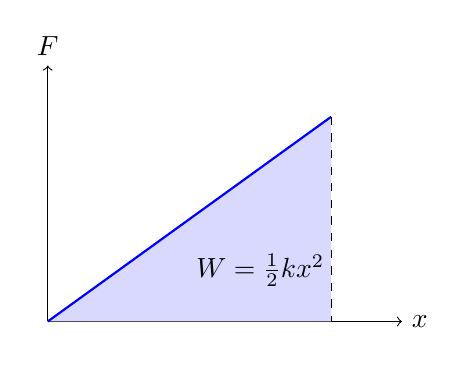
\begin{tikzpicture}[x=.9cm,y=.65cm]\draw[->](0,0)--(5,0)node[right]{$x$};\draw[->](0,0)--(0,5)node[above]{$F$};\fill[blue!15](0,0)--(4,4)--(4,0)--cycle;\draw[thick,blue](0,0)--(4,4);\draw[dashed](4,4)--(4,0);\node at (3,1){$W=\frac12kx^2$};\end{tikzpicture}
\end{center}
\section{Ví dụ có lời giải}
\subsection*{Ví dụ 3.1}
Gia tốc a=2t, ban đầu v=3 m/s và x=1 m. Tìm v(t), x(t), x(2).

\textbf{Lời giải.} $v=3+\int_0^t2s\,ds=3+t^2$. $x=1+\int_0^t(3+s^2)\,ds=1+3t+t^3/3$. Tại 2 s, $x=1+6+8/3=29/3$ m.
\subsection*{Ví dụ 3.2}
Lực F(x)=4x+3 N dọc trục x từ 0 đến 2 m. Tính công và lực trung bình theo quãng đường.

\textbf{Lời giải.} $W=\int_0^2(4x+3)dx=[2x^2+3x]_0^2=14$ J. Lực trung bình theo quãng đường $W/2=7$ N.
\subsection*{Ví dụ 3.3}
Thanh từ x=0 đến L có mật độ dài \ensuremath{\lambda}(x)=\ensuremath{\lambda}\textsubscript{0}x/L. Tìm khối lượng và khối tâm.

\textbf{Lời giải.} $m=(\lambda_0/L)\int_0^L x\,dx=\lambda_0L/2$. Moment bậc nhất $(\lambda_0/L)\int_0^Lx^2dx=\lambda_0L^2/3$. Vậy $x_{\rm cm}=2L/3$, lệch về đầu đậm đặc hơn.
\section{Nhiệm vụ thực nghiệm}
Xấp xỉ công của F=4x+3 trên 0\ensuremath{\le}x\ensuremath{\le}2 bằng hình chữ nhật trái và phải với 4, 8, 16 khoảng. So sánh với 14 J và giải thích vì sao hai tổng kẹp kết quả đúng khi lực tăng.
\section{Ứng dụng hiện đại và chuyển giao}
Cảm biến điện lấy dòng $I(t)=0{,}1e^{-t/5}$ A từ nguồn ổn áp 3 V trong 10 s. Điện lượng $Q=\int_0^{10}I(t)dt=0{,}5(1-e^{-2})\approx0{,}432$ C. Năng lượng cấp $E=3Q\approx1{,}30$ J. Chuyển giao: nếu điện áp biến thiên, phải tính năng lượng $\int U(t)I(t)dt$, không nhân hai giá trị trung bình thời gian độc lập.
\section{Chỉ dẫn đọc nguồn}
SW-1.3.1–1.3.5: pp. 35–49; SJ-03: pp. 12–14; SJ-20: pp. 86–89; JP-A: mathematical physics appendix.
\section{Luyện tập độc lập}
\begin{enumerate}
\item \textbf{PHY201-A-3.1}. Tích phân v=4-2t trên 0\ensuremath{\le}t\ensuremath{\le}4. Tìm độ dời và quãng đường.
\item \textbf{PHY201-A-3.2}. Lò xo k=80 N/m. Tính công của lực lò xo từ x=0,1 đến 0,3 m.
\item \textbf{PHY201-A-3.3}. Thanh mảnh đều dài L, khối lượng m, quay quanh trục vuông góc qua một đầu. Suy ra I.
\item \textbf{PHY201-A-3.4}. Tính \ensuremath{\int}\textsubscript{0}¹ 2x/(1+x\textsuperscript{2}) dx và nêu phép đổi biến.
\item \textbf{PHY201-A-3.5}. Với F(x)=kx\textsuperscript{2}, k>0, suy công từ 0 đến L và đơn vị của k.
\end{enumerate}
\chapter{Xấp xỉ Taylor, phân tích thứ nguyên và tọa độ cực}
\section{Mục tiêu và chẩn đoán}
Dùng tham số nhỏ không thứ nguyên, lý giải sai số xấp xỉ, suy ra vận tốc và gia tốc tọa độ cực.

\textbf{Dự đoán:} Vì sao xấp xỉ góc nhỏ chỉ có ý nghĩa sau khi quy định radian?
\section{Lý thuyết và suy dẫn}
Khai triển Taylor quanh $x_0$: $f(x_0+h)=f(x_0)+hf'(x_0)+h^2f''(x_0)/2+\cdots$ khi thỏa điều kiện trơn và hội tụ tương ứng. Xấp xỉ bậc nhất chỉ cục bộ. Với tham số nhỏ không thứ nguyên $\epsilon$, $(1+\epsilon)^n\approx1+n\epsilon$; số hạng tiếp là $n(n-1)\epsilon^2/2$. Với radian, $\sin\theta\approx\theta$, $\cos\theta\approx1-\theta^2/2$. Với $\theta$ thực, sai số tuyệt đối xấp xỉ sin bậc nhất bị chặn bởi $|\theta|^3/6$. Chọn dung sai trước khi quyết định cắt.

Phân tích thứ nguyên ràng buộc số mũ. Giả sử chu kỳ con lắc đơn chỉ phụ thuộc chiều dài $l$ và gia tốc trọng trường $g$: $T=C l^a g^b$. So số mũ thời gian $-2b=1$, nên $b=-1/2$; số mũ độ dài $a+b=0$, suy $a=1/2$. Vậy $T=C\sqrt{l/g}$. Động lực học góc nhỏ cho $C=2\pi$; thứ nguyên không tự xác định hệ số hay loại trừ phụ thuộc biên độ không thứ nguyên. Phải có căn cứ chọn biến của mô hình.

Trong tọa độ cực phẳng $\vec r=r\hat e_r$, với $\hat e_r=(\cos\theta,\sin\theta)$, $\hat e_\theta=(-\sin\theta,\cos\theta)$. Đạo hàm cho $\dot{\hat e}_r=\dot\theta\hat e_\theta$, $\dot{\hat e}_\theta=-\dot\theta\hat e_r$. Do đó $\vec v=\dot r\hat e_r+r\dot\theta\hat e_\theta$ và $\vec a=(\ddot r-r\dot\theta^2)\hat e_r+(r\ddot\theta+2\dot r\dot\theta)\hat e_\theta$. Các số hạng do cơ sở thay đổi; bỏ đạo hàm cơ sở sẽ mất thành phần hướng tâm và số hạng chéo. Chuyển động tròn đều có $\dot r=\ddot r=\ddot\theta=0$ và $a_r=-r\omega^2$.

Với tích phân trường và thể tích, phần tử diện tích cực $dA=r\,dr\,d\theta$; thể tích trụ $dV=r\,dr\,d\theta\,dz$; thể tích cầu $dV=r^2\sin\theta\,dr\,d\theta\,d\phi$ với $\theta$ là góc cực. Các hệ số biểu diễn độ giãn hình học ô tọa độ. Ví dụ $\int_0^{2\pi}\int_0^R r\,dr\,d\theta=\pi R^2$. Giải tích vector đầy đủ là nội dung mở rộng sau.
\begin{center}
\begin{tikzpicture}[scale=.85]\draw[->](0,0)--(5,0)node[right]{$x$};\draw[->](0,0)--(0,4)node[above]{$y$};\draw[gray](0,0)circle(2.5);\draw[->,thick](0,0)--(2,1.5)node[midway,above left]{$r$};\draw[->,blue,very thick](2,1.5)--(3.2,2.4)node[right]{$\hat e_r$};\draw[->,orange,very thick](2,1.5)--(1.1,2.7)node[above]{$\hat e_\theta$};\draw(.9,0)arc(0:36.87:.9);\node at(1.2,.35){$\theta$};\end{tikzpicture}
\end{center}
\section{Ví dụ có lời giải}
\subsection*{Ví dụ 4.1}
Với \ensuremath{\theta}=0,2 rad, ước lượng sin \ensuremath{\theta} bậc nhất và bậc ba; chặn sai số tuyệt đối bậc nhất.

\textbf{Lời giải.} Bậc nhất 0,2. Bậc ba $0{,}2-0{,}2^3/6=0{,}1986667$. Cận $0{,}2^3/6=0{,}0013333$. Giá trị $\sin0{,}2\approx0{,}1986693$, phù hợp.
\subsection*{Ví dụ 4.2}
Giả sử tốc độ sóng chỉ phụ thuộc áp suất p và khối lượng riêng \ensuremath{\rho}. Suy ra dạng theo thứ nguyên.

\textbf{Lời giải.} $v=Cp^a\rho^b$. Thứ nguyên: $ML^{-1}T^{-2}$ và $ML^{-3}$. So sánh cho $a+b=0$, $-2a=-1$, $-a-3b=1$. Vậy $a=1/2,b=-1/2$, $v=C\sqrt{p/\rho}$. Mô hình âm đoạn nhiệt trong khí lý tưởng cho $C=\sqrt\gamma$.
\subsection*{Ví dụ 4.3}
Hạt có r=2+t (m), \ensuremath{\theta}=3t (rad). Tìm các thành phần vận tốc và gia tốc cực tại t=1 s.

\textbf{Lời giải.} Tại t=1, $r=3$, $\dot r=1$, $\ddot r=0$, $\dot\theta=3$, $\ddot\theta=0$. Vậy $(v_r,v_\theta)=(1,9)$ m/s và $(a_r,a_\theta)=(-27,6)$ m/s$^2$.
\section{Nhiệm vụ thực nghiệm}
Đo chu kỳ con lắc ở biên độ khoảng 5\textdegree{}, 15\textdegree{}, 30\textdegree{} bằng vật nhẹ và biên độ thấp. So sánh với chu kỳ góc nhỏ; thảo luận bất định thời gian và vì sao không phát hiện chênh lệch không chứng minh chu kỳ độc lập biên độ.
\section{Ứng dụng hiện đại và chuyển giao}
Gần đáy giếng thế trơn, $U(x)\approx U(0)+kx^2/2$ khi $U'(0)=0$, $k=U''(0)>0$. Lực $F\approx-kx$; do đó li độ nhỏ tuân theo dao động điều hòa. Xấp xỉ cục bộ này quan trọng trong dao động mạng tinh thể và cảm biến cộng hưởng. Chuyển giao: với $U=U_0+kx^2/2+\beta x^4/4$, so sánh độ lớn lực phi tuyến và tuyến tính tại biên độ A. Tỉ số $|\beta|A^2/k$; nếu không nhỏ, mô hình điều hòa không phù hợp.
\section{Chỉ dẫn đọc nguồn}
SW-1.2.6: pp. 31–32; SW-1.3.5: p. 49; JP-A: pp. 323–337; JP-1.5: p. 8; SJ-15: pp. 56–59; SJ-22: pp. 92–94.
\section{Luyện tập độc lập}
\begin{enumerate}
\item \textbf{PHY201-A-4.1}. Ước lượng (1,04)^(1/2) đến bậc hai và so sánh bậc nhất.
\item \textbf{PHY201-A-4.2}. Dùng cận \ensuremath{\theta}\textsuperscript{3}/6 tìm giới hạn góc dương đủ để sai số tuyệt đối xấp xỉ sin \ensuremath{\le}0,001.
\item \textbf{PHY201-A-4.3}. Giả sử lực cản chỉ phụ thuộc khối lượng riêng \ensuremath{\rho}, tốc độ v và diện tích A. Xác định dạng đơn thức theo thứ nguyên.
\item \textbf{PHY201-A-4.4}. Với r=0,5 m và \ensuremath{\theta}=4t, tìm tốc độ và độ lớn gia tốc.
\item \textbf{PHY201-A-4.5}. Suy diện tích vành khuyên bán kính trong a, ngoài b bằng tích phân cực.
\end{enumerate}
\chapter*{Tài liệu tham khảo và mô phỏng}
Swiss Physics Olympiad Script, 3rd ed. (2019).\par
The Committee of Japan Physics Olympiad (2014). \textit{Physics Olympiad: Basic to Advanced Exercises}. World Scientific.\par
Tan Chien Hao (2024). \textit{Freshman Physics}.\par
\url{https://diavn.github.io/truongchuyen/physics-curriculum.html}\par
\url{https://diavn.github.io/truongchuyen/physics-math-lab.html}
\appendix
\chapter{Lời giải đầy đủ phần luyện tập}
\section{Vector, phép chiếu và các tích vật lý}
\begin{enumerate}
\item \textbf{PHY201-A-1.1}. Vô hướng $a\cdot n=24/5$; vector $(24/5)n=(72/25,96/25,0)$. Phần còn lại có tích vô hướng với n bằng 0.
\item \textbf{PHY201-A-1.2}. $\vec a\times\vec b=(-5,1,1)$. Tích với a: $-5+2+3=0$; với b: $1-1=0$.
\item \textbf{PHY201-A-1.3}. $P=-5-8=-13$ W. Lực này lấy đi năng lượng cơ học tại thời điểm đó (lực khác có thể cấp năng lượng).
\item \textbf{PHY201-A-1.4}. $\vec v\times\vec B=(0,-600,0)$; nhân $2\times10^{-6}$ C: $\vec F=(0,-1{,}2\times10^{-3},0)$ N. Tích vô hướng với v bằng 0.
\item \textbf{PHY201-A-1.5}. Quanh gốc $\tau_z=0{,}2(0)-0{,}3(10)=-3$ N m. Quanh O\ensuremath{\prime}, vị trí tương đối $(0{,}2,0,0)$ song song F nên moment bằng 0.
\end{enumerate}
\section{Đạo hàm: tốc độ biến thiên, cực trị và mô hình cục bộ}
\begin{enumerate}
\item \textbf{PHY201-A-2.1}. $v=4-2t=0$ tại $t=2$ s; dấu đổi dương sang âm. $a=-2$ m/s$^2$.
\item \textbf{PHY201-A-2.2}. $a=-2e^{-t/3}$ m/s$^2$; $a(0)=-2$, $a(3)=-2/e\approx-0{,}736$ m/s$^2$.
\item \textbf{PHY201-A-2.3}. $K=v^2=9t^4$ J, $K(2)=144$ J; $dK/dt=36t^3=288$ W tại 2 s. Kiểm tra $Fv=2(12)(12)=288$ W.
\item \textbf{PHY201-A-2.4}. $P'=12-4I=0$ tại $I=3$ A, $P''=-4$. Các giá trị $P(0)=0$, $P(3)=18$, $P(4)=16$ W. Cực đại 18 W.
\item \textbf{PHY201-A-2.5}. $[(t+h)^3-(t-h)^3]/(2h)=3t^2+h^2$. Đạo hàm đúng $3t^2$; sai số cắt cụt $h^2$ trong hệ đơn vị đã chọn. Giảm h một nửa làm sai số giảm bốn lần.
\end{enumerate}
\section{Tích phân, tích lũy và điều kiện đầu}
\begin{enumerate}
\item \textbf{PHY201-A-3.1}. Vận tốc bằng 0 tại t=2. $\int_0^4(4-2t)dt=0$; diện tích dương 4 m, âm -4 m, quãng đường 8 m.
\item \textbf{PHY201-A-3.2}. $W=\int_{0.1}^{0.3}-80x\,dx=-40(0{,}09-0{,}01)=-3{,}2$ J. Thế năng tăng 3,2 J.
\item \textbf{PHY201-A-3.3}. $dm=(m/L)dx$. $I=(m/L)\int_0^L x^2dx=mL^2/3$.
\item \textbf{PHY201-A-3.4}. $u=1+x^2$, $du=2x\,dx$. Cận 1 và 2, tích phân $\int_1^2du/u=\ln2$.
\item \textbf{PHY201-A-3.5}. $W=kL^3/3$. Vì F theo N và x\textsuperscript{2} theo m\textsuperscript{2}, đơn vị k là N/m$^2$. Công có đơn vị N m.
\end{enumerate}
\section{Xấp xỉ Taylor, phân tích thứ nguyên và tọa độ cực}
\begin{enumerate}
\item \textbf{PHY201-A-4.1}. $\sqrt{1+\epsilon}\approx1+\epsilon/2-\epsilon^2/8$. Tại 0,04: bậc nhất 1,02; bậc hai 1,0198. Giá trị đúng khoảng 1,0198039.
\item \textbf{PHY201-A-4.2}. $\theta^3/6\le0{,}001$ cần $\theta\le(0{,}006)^{1/3}\approx0{,}1817$ rad, khoảng $10{,}4^\circ$. Đây là điều kiện đủ, không khẳng định cần.
\item \textbf{PHY201-A-4.3}. $F=C\rho^a v^b A^c$. Khối lượng cho $a=1$, thời gian $b=2$, độ dài $-3+2+2c=1$ nên $c=1$. Vậy $F=C\rho v^2 A$; hệ số thực phụ thuộc hình dạng, số Reynolds và chế độ dòng.
\item \textbf{PHY201-A-4.4}. $v=r\omega=2$ m/s; $a=r\omega^2=8$ m/s$^2$, hướng tâm.
\item \textbf{PHY201-A-4.5}. $A=\int_0^{2\pi}\int_a^b r\,dr\,d\theta=2\pi(b^2-a^2)/2=\pi(b^2-a^2)$. Kiểm tra đúng khi a=0 và a=b.
\end{enumerate}
\end{document}
